\chapter{Introduction}

L'objectif de ce rapport est de présenter la conception de notre interface homme-machine. Elle s'inscrit dans le cadre du projet multi-module du master 2 alma. Ce livrable est structuré selon la méthode de conception LUCID (Logical User-Centered Interactive Design) et se décompose donc en 5 parties.

\begin{enumerate}
 \item Développement du concept de produit
 \item Analyse
 \item Conception initiale de l’interface
 \item Implémentation de l’application
 \item Évaluation
\end{enumerate}



\chapter{Présentation de l'architecture}



La partie qui nous concerne ici correspond à l'interface du client Web de l'architecture suivante :

\begin{figure}[H]
\begin{center}
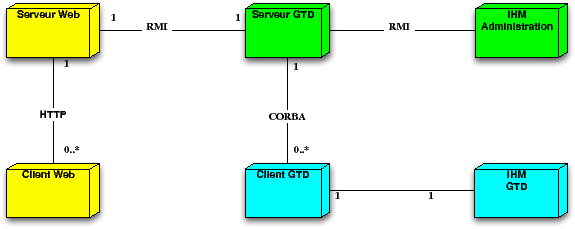
\includegraphics[scale=0.8]{diagrams/archi.png}
\caption{Architecture Générale}
\end{center}
\end{figure}


L'objectif ce cette IHM est de gérer deux types de serveurs GTD (Getting things done) : un premier réalisé par une équipe du master2 alma, un second disponible gratuitement sur internet, nommé ToodleDo\footnote{http://www.toodledo.com}.

\chapter{Etape 1 : Développement du concept de produit}


\section{Objectifs du projet}
Le projet s'inscrit dans un cadre universitaire, ainsi il n'est pas destiné à être commercialisé. Cependant, ce projet est sous licence GPL3 et peut donc être distribué, et modifié librement. Aucune contrainte de conception n'est définie pour l'IHM, hormis le fait qu'elle doit respecter scrupuleusement la définition des fonctionnalités de la méthode GTD.


\section{Contraintes de l'IHM}
Le logiciel doit être utilisable facilement par n'importe quels types d'utilisateurs, il devra respecter les contraintes suivantes : \\
\begin{description}
 \item[Facilité de prise en main, intuitivité :] Le logiciel ne disposera pas de fonctions trop avancées pour ne pas déstabiliser l'utilisateur et pour gagner un maximum de temps, en allant à l'essentiel.
 \item[Aide en ligne :] Le logiciel disposera de bulle d'aide (tooltips) pour aider l'utilisateur de façon ponctuelle. Une documentation papier ainsi qu'une formation seront également mis à disposition de l'utilisateur.
 \item[Textes en anglais et français :] Internationalisation pour élargir le panel d'utilisateurs. Dans un premier temps, seul l'anglais et le français seront disponibles.
 \item[Respect de la méthode GTD :] Le cahier des charges de l'application a été respecté. Ceci est détaillé dans le livrable de l'analyse du projet.
 \item[Respect des bonnes pratiques de conception des IHM] Le logiciel respectera les conventions de base de toute Interface Homme Machine (Taille des boutons, disposition des menu en haut, lecture de l'IHM de gauche à droite...)
 \item[Rapidité de fonctionnement :] L'IHM sera réactive. Cependant en cas de traitements longs, l'utilisateur sera averti du temps restant. Cela permet de faire patienter l'utilisateur, sans lui laisser croire que l'application ne réponds plus.
\end{description}


\section{Utilisateurs}
Le produit s'adresse à tous les types d'utilisateurs disposant des compétences de bases en informatique. Ainsi, ceux-ci doivent être en mesure de savoir naviguer sur internet et de savoir manipuler un logiciel relativement simple. 

\section{Fonctionnalités principales}
L'objectif du projet est de fournir un logiciel complet de gestion de tâches et s'appuyant sur la méthode GTD\footnote{http://fr.wikipedia.org/wiki/Getting\_Things\_Done}. Le logiciel est multi-utilisateurs et est en mesure de fonctionner grâce à deux serveurs : \\
\begin{itemize}
 \item Un serveur GTD créé par un groupe du master alma
 \item Un serveur ToodleDo\\
\end{itemize}

Il devra donc permettre la création de tâches, de projets, de contextes, etc... De plus, il devra permettre d'effectuer une synchronisation des données entre les deux serveurs, dans le cas où les deux serveurs ne seraient pas synchronisés. Ce genre de scénarios se produit par exemple lorsqu'un serveur est indisponible lors d'une mise à jour.





\chapter{Etape 2 : Analyse}

\section{Segmentation des utilisateurs}
Comme nous l'avons dit, le logiciel sera utilisable par n'importe quels types d'utilisateurs. C'est pourquoi il n'y aura pas différentes classes d'utilisateurs pour l' IHM. Cependant pour le reste du système (Serveur GTD notamment) une classe administrateur est définie. Elle dispose des droits maximums sur le système et offre la possibilité d'administrer le serveur. Cette classe ne fait pas partie de notre projet (seulement sur le serveur GTD) et n'est donc pas décrite dans la suite du document.

\section{Principales fonctionnalités}
Les fonctionnalités de l'IHM respectent les principes de la méthode GTD. Ainsi, on retrouve les activités principales suivantes : \\
\begin{itemize}
 \item Collecte des informations : Création de notes (idées) qui vont aboutir à la création de tâches
 \item Création des tâches
 \item Organisation des tâches : Manipulation des tâches et des projets
 \item Mise à jour des tâches
 \item Visualisation : Affichage des tâches selon le contexte
\end{itemize}




\section{Scénarios de l'IHM}

Voici une liste exhaustive des fonctionnalités offertes par le logiciel. L'ensemble des scénarios s'appuient sur des cas d'utilisations cockburn.

\subsection{Identification}

\begin{usecase}{Identification}

\begin{information}
\item[Acteur: ] Utilisateur
\item[Niveau:] Tâche principale
\item[Portée:] IHM, Base de données 
\item[Pré-condition:] L'utilisateur est non connecté et déjà inscrit. 
\item[Post-condition:] L'utilisateur est connecté. 
\item[Priorité:] (5/5) : Cette étape est nécessaire pour chacun des prochains cas d'utilisation.
\item[Fréquence:] Chaque lancement d'application.	
\end{information}	

\begin{scenario}
\item[1] L'utilisateur entre sont identifiant et son mot de passe,
\item[2] Il valide,
\item[3] L'utilisateur est connecté. 
\end{scenario}	

\begin{extension}
	\item[1]Renvoyer le mot de passe
	\item[2]Création d'un compte
\end{extension}
\end{usecase}


\subsubsection{Exigences fonctionnelles}
%<Itemize the detailed functional requirements associated with this feature. These are the software capabilities that must be present in order for the user to carry out the services provided by the feature, or to execute the use case. Include how the product should respond to anticipated error conditions or invalid inputs. Requirements should be concise, complete, unambiguous, verifiable, and necessary. Use “TBD” as a placeholder to indicate when necessary information is not yet available.>

%<Each requirement should be uniquely identified with a sequence number or a meaningful tag of some kind.>

%REQ-1:	
%REQ-2:
\begin{itemize}	\renewcommand{\labelitemi}{}
	\item \textbf{FONC11} - Saisie des identifiants,
	\item \textbf{FONC12} - Connexion (avec gestion de session),
	\item \textbf{FONC13} - Inscription,
	\item \textbf{FONC14} - Régénération de mot de passe.\\
\end{itemize}

\subsection{Collecte des informations}

L'application n'a normalement pas à intervenir dans cette étape. Le recensement des idées est effectivement un processus utilisateur. Cependant, un pense-bête a idées non traitées par l'utilisateur peut s'avérer fort utile dans le cas où l'utilisateur est interrompu dans son processus.Un pense bête permet alors de stocker les idées non traitées.

\begin{usecase}{Collect}

\begin{information}
\item[Acteur:] Utilisateur
\item[Niveau:] Tâche principale
\item[Portée:] IHM, Base de donnée
\item[Partie prenante et intérêt :]
	Le recensement exhaustif de tout ce qui peut justifier une quelconque intervention de notre part : en suspens, inachèvement, en attente, intention, projet, manque, usure, mauvais fonctionnement, problème, in- satisfaction, besoin, engagements à tenir,etc.
Exemples : cette carte de visite restée dans une poche, cette facture dans la boîte à gants, cette demande reçue, ce dossier qui traîne sur le bureau, cette agrafeuse qui coince, cette course à faire, ce problème à résoudre, cette suggestion à tester, les messages de la boîte vocale, ce projet jamais réalisée, ce souci de santé, ce fauteuil qui grince, les performances de ce collaborateur, toutes ces choses en retard...
\item[Pré-condition:] Aucune. 
\item[Post-condition:] Les informations sont enregistrées dans l'application.
\item[Priorité:] (1/5) : Cette étape n'est pas indispensable, et peut être effectuer sans l'aide du système informatique.
\item[Fréquence:] Chaque début de journée.
\end{information}	

\begin{scenario}
\item[1] L'utilisateur après avoir effectuer sa réflexion, saisie les informations qu'il à recensée dans la boite à idée de l'application.
\end{scenario}

%\begin{extension}
%\item[1] 
%\end{extension}
	
\end{usecase}

% Utilisez le canevas de cockburn pour décrire le cas d'utilisation
% Indiquez la priotité: Haute, Moyenne et Basse
% Indiquez, éventuellement, des mesures spécifiques, comme le profit, le coût, les risques, etc. 
% (sur une échelle relative d'un minimum de 1 à un maximum de 9))

\subsubsection{Exigences fonctionnelles}

\begin{itemize}	\renewcommand{\labelitemi}{}
\item \textbf{FONC21} - Saisie des idées,
\item \textbf{FONC22} - Stockage des idées,
\item \textbf{FONC23} - Suppression des idées.
\end{itemize}


\subsection{Organisation des tâches}
	\begin{usecase}{Organize} 
		\begin{information}
			\item[Acteur :] Utilisateur
			\item[Niveau :] Tâche principale
			\item[Portée :] IHM, base de données
			\item[Pré-condition :] On dispose d''une liste de tâches issues de l'organisation des données.
			\item[Post-condition :] Les tâches appartiennent ou non à un projet, sont organisées en séquence ou non.
			\item[Priorité :] Haute
			\item[Fréquence :] Après chaque traitement des données.
		\end{information}
		\begin{scenario}
			\item[1] L'utilisateur regroupe les tâches par projet en fonction des propriétés communes de leurs contextes et de leurs intérêts communs.
			\item[1] Il peut aussi séquencer les tâches d'un projet. 
			\item[2] Il a aussi la possibilité de créer des sous-projets afin de donner un aspect hiérarchique au projet principal.
		\end{scenario}
		\begin{extension}
			\item[1]Si une tâche est isolée, elle n'appartient à aucun projet et n'est pas séquençable.
		\end{extension}
	\end{usecase}
		
	\subsubsection{Exigences fonctionnelles}
		Pour regrouper les tâches l'utilisateur doit pouvoir :
		\begin{itemize}	\renewcommand{\labelitemi}{}
			\item \textbf{FONC31} - créer/modifier/supprimer des projets,
			\item \textbf{FONC33} - affecter ou non des tâches à un projet,
			\item \textbf{FONC35} - affecter ou non des projets à un projet (sous-projets).
		\end{itemize}
		
	\subsubsection{Exigences non-fonctionnelles}
		\begin{itemize}	\renewcommand{\labelitemi}{}
			\item \textbf{FONC36} - Les tâches et sous-projets d'un même projet doivent participer à un même but.
			\item \textbf{FONC37} - Les tâches d'une même séquence doivent appartenir au même projet.
			\item \textbf{FONC38} - Les tâches et sous-projets d'un même projet doivent avoir des propriétés communes dans leurs contextes respectif.			
		\end{itemize}
		

\subsection{Affichage des tâches}
	\begin{usecase}{Affichage des tâches} 
		\begin{information}
			\item[Acteur :] Utilisateur
			\item[Niveau :] Tâche principale
			\item[Portée :] IHM
			\item[Pré-condition :] On dispose d'une liste de tâches, de contextes, de projets...
			\item[Post-condition :] Les tâches sont affichées selon les critères et vues choisies par l'utilisateur.
			\item[Priorité :] Haute
			\item[Fréquence :] Selon les besoins de l'utilisateur.
		\end{information}
		\begin{scenario}
			\item[1] L'utilisateur affiche les tâches qu'il effectuera selon les projets qu'il a choisit et le contexte courant.
			\item[2] Les tâches sont présentées de différentes manières (échéancier, agenda...).
		\end{scenario}
	\end{usecase}
	
	\subsubsection{Exigences fonctionnelles}
		L'utilisateur doit pouvoir via l'IHM :
		\begin{itemize}	\renewcommand{\labelitemi}{}
			\item \textbf{FONC71}- choisir les projets à réaliser.
			\item \textbf{FONC72}- sélectionner la ou les vues dans lesquelles seront affichées les tâches (échéancier, agenda...).
		\end{itemize}
		
\subsection{Réactualisation des tâches}
	\begin{usecase}{Réactualisation des tâches} 
		\begin{information}
			\item[Acteur :] Utilisateur
			\item[Niveau :] Tâche principale
			\item[Portée :] IHM, base de données
			\item[Pré-condition :] On dispose d''une liste de tâches.
			\item[Post-condition :] On délègue des tâches, celles finies sont supprimées, les vues sont mises à jour suivant le nouveau contexte, création automatique des tâches périodiques.
			\item[Priorité :] Haute
			\item[Fréquence :] Au moins une fois par jour.
		\end{information}
		\begin{scenario}
			\item[1] L'utilisateur change le contexte courant.
			\item[2] Indique les tâches effectuées.
			\item[3] Délègue des tâches.
		\end{scenario}
		\begin{extension}
			\item[2b] L'utilisateur peut annuler ses modifications.
		\end{extension}
	\end{usecase}
		
	
	\subsection{Exigences fonctionnelles}
		L'utilisateur doit pouvoir :
		\begin{itemize}	\renewcommand{\labelitemi}{}
			\item \textbf{FONC41} - mettre à jour le contexte.
			\item \textbf{FONC42} - indiquer les tâches réalisées.
			\item \textbf{FONC43} - déléguer une tâche.
			\item \textbf{FONC44} - revenir en arrière.
		\end{itemize}

		
%%%%%%%%%%%%%%%%%%%%%%%%%%%%%%%%%%%%%%%%%%%%%%%%%%%%%%%%%%%%%%%%%%%%%%%%%%%%%%%%%%%%%%%%%%%%%%%%%%%%%%%%%%%%%%%%%%%%%%%%%%%%%%%%%%%%%%%%%%%%%%%%%%%%%%%%%%%%
	
		
		
		
		
\subsection{Traitement des informations}
\begin{usecase}{Process}

\begin{information}
\item[Acteur: ] Utilisateur
\item[Niveau:] Tâche principale
\item[Portée:] IHM, Base de donnée 
\item[Pré-condition:] L'utilisateur est connecté au serveur web. 
\item[Post-condition:] Une tâche est créée sur les serveur GTD et ToodleDo. 
\item[Priorité:] (5/5) : Cette étape est nécessaire pour chacun des prochains cas d'utilisation.
\item[Fréquence:] De façon ponctuelle.	
\end{information}	

\begin{scenario}
\item[1] L'utilisateur regarde les éléments affichés dans sa boite à idées.
\item[2] L'utilisateur saisie les informations relatives à la tâche qu'il souhaite créer (nom, date debut, date fin, priorité, temps et energie requis ...).
\item[3] L'utilisateur crée la tâche.
\end{scenario}	

\begin{extension}
	\item[1]L'utilisateur oublie de remplir un champ obligatoire.
\end{extension}
\end{usecase}

\subsubsection{Exigences fonctionnelles}
%<Itemize the detailed functional requirements associated with this feature. These are the software capabilities that must be present in order for the user to carry out the services provided by the feature, or to execute the use case. Include how the product should respond to anticipated error conditions or invalid inputs. Requirements should be concise, complete, unambiguous, verifiable, and necessary. Use “TBD” as a placeholder to indicate when necessary information is not yet available.>

%<Each requirement should be uniquely identified with a sequence number or a meaningful tag of some kind.>

%REQ-1:	
%REQ-2:
\begin{itemize}	\renewcommand{\labelitemi}{}
	\item \textbf{FONC51} - Affichage de la boite à idées,
	\item \textbf{FONC52} - Saisie des informations relatives à une tâche,
	\item \textbf{FONC53} - Création d'une tâche,
\end{itemize}







\subsection{Synchronisation}
\begin{usecase}{Synchronisation}

\begin{information}
\item[Acteur: ] Serveur Web
\item[Niveau:] Tâche principale
\item[Portée:] Serveur GTD et ToodleDo et Serveur Web
\item[Pré-condition:] Le serveur web n'est pas synchronisé avec le serveur GTD ni ToodleDo
\item[Post-condition:] Le serveur web et les serveurs GTD et ToodleDo sont synchronisés
\item[Priorité:] (5/5) : Cette étape est nécessaire pour assurer une persistance des informations.
\item[Fréquence:] A chacune des transactions
\end{information}	

\begin{scenario}
\item[1] L'utilisateur effectue une opération sur le client web
\item[2] Le serveur web enregistre les modifications utilisateur en mettant à jour sa base de données
\item[3] Le serveur web envoi les modifications effectuées aux serveurs
\end{scenario}	

\begin{extension}
	\item[1]La connexion entre les serveurs web et GTD et/ou ToodleDo est interrompue
	\item[2]La connexion entre les serveurs web et GTD et/ou ToodleDo se rétablie
\end{extension}
\end{usecase}

  \begin{figure}[H]
  \begin{center}
  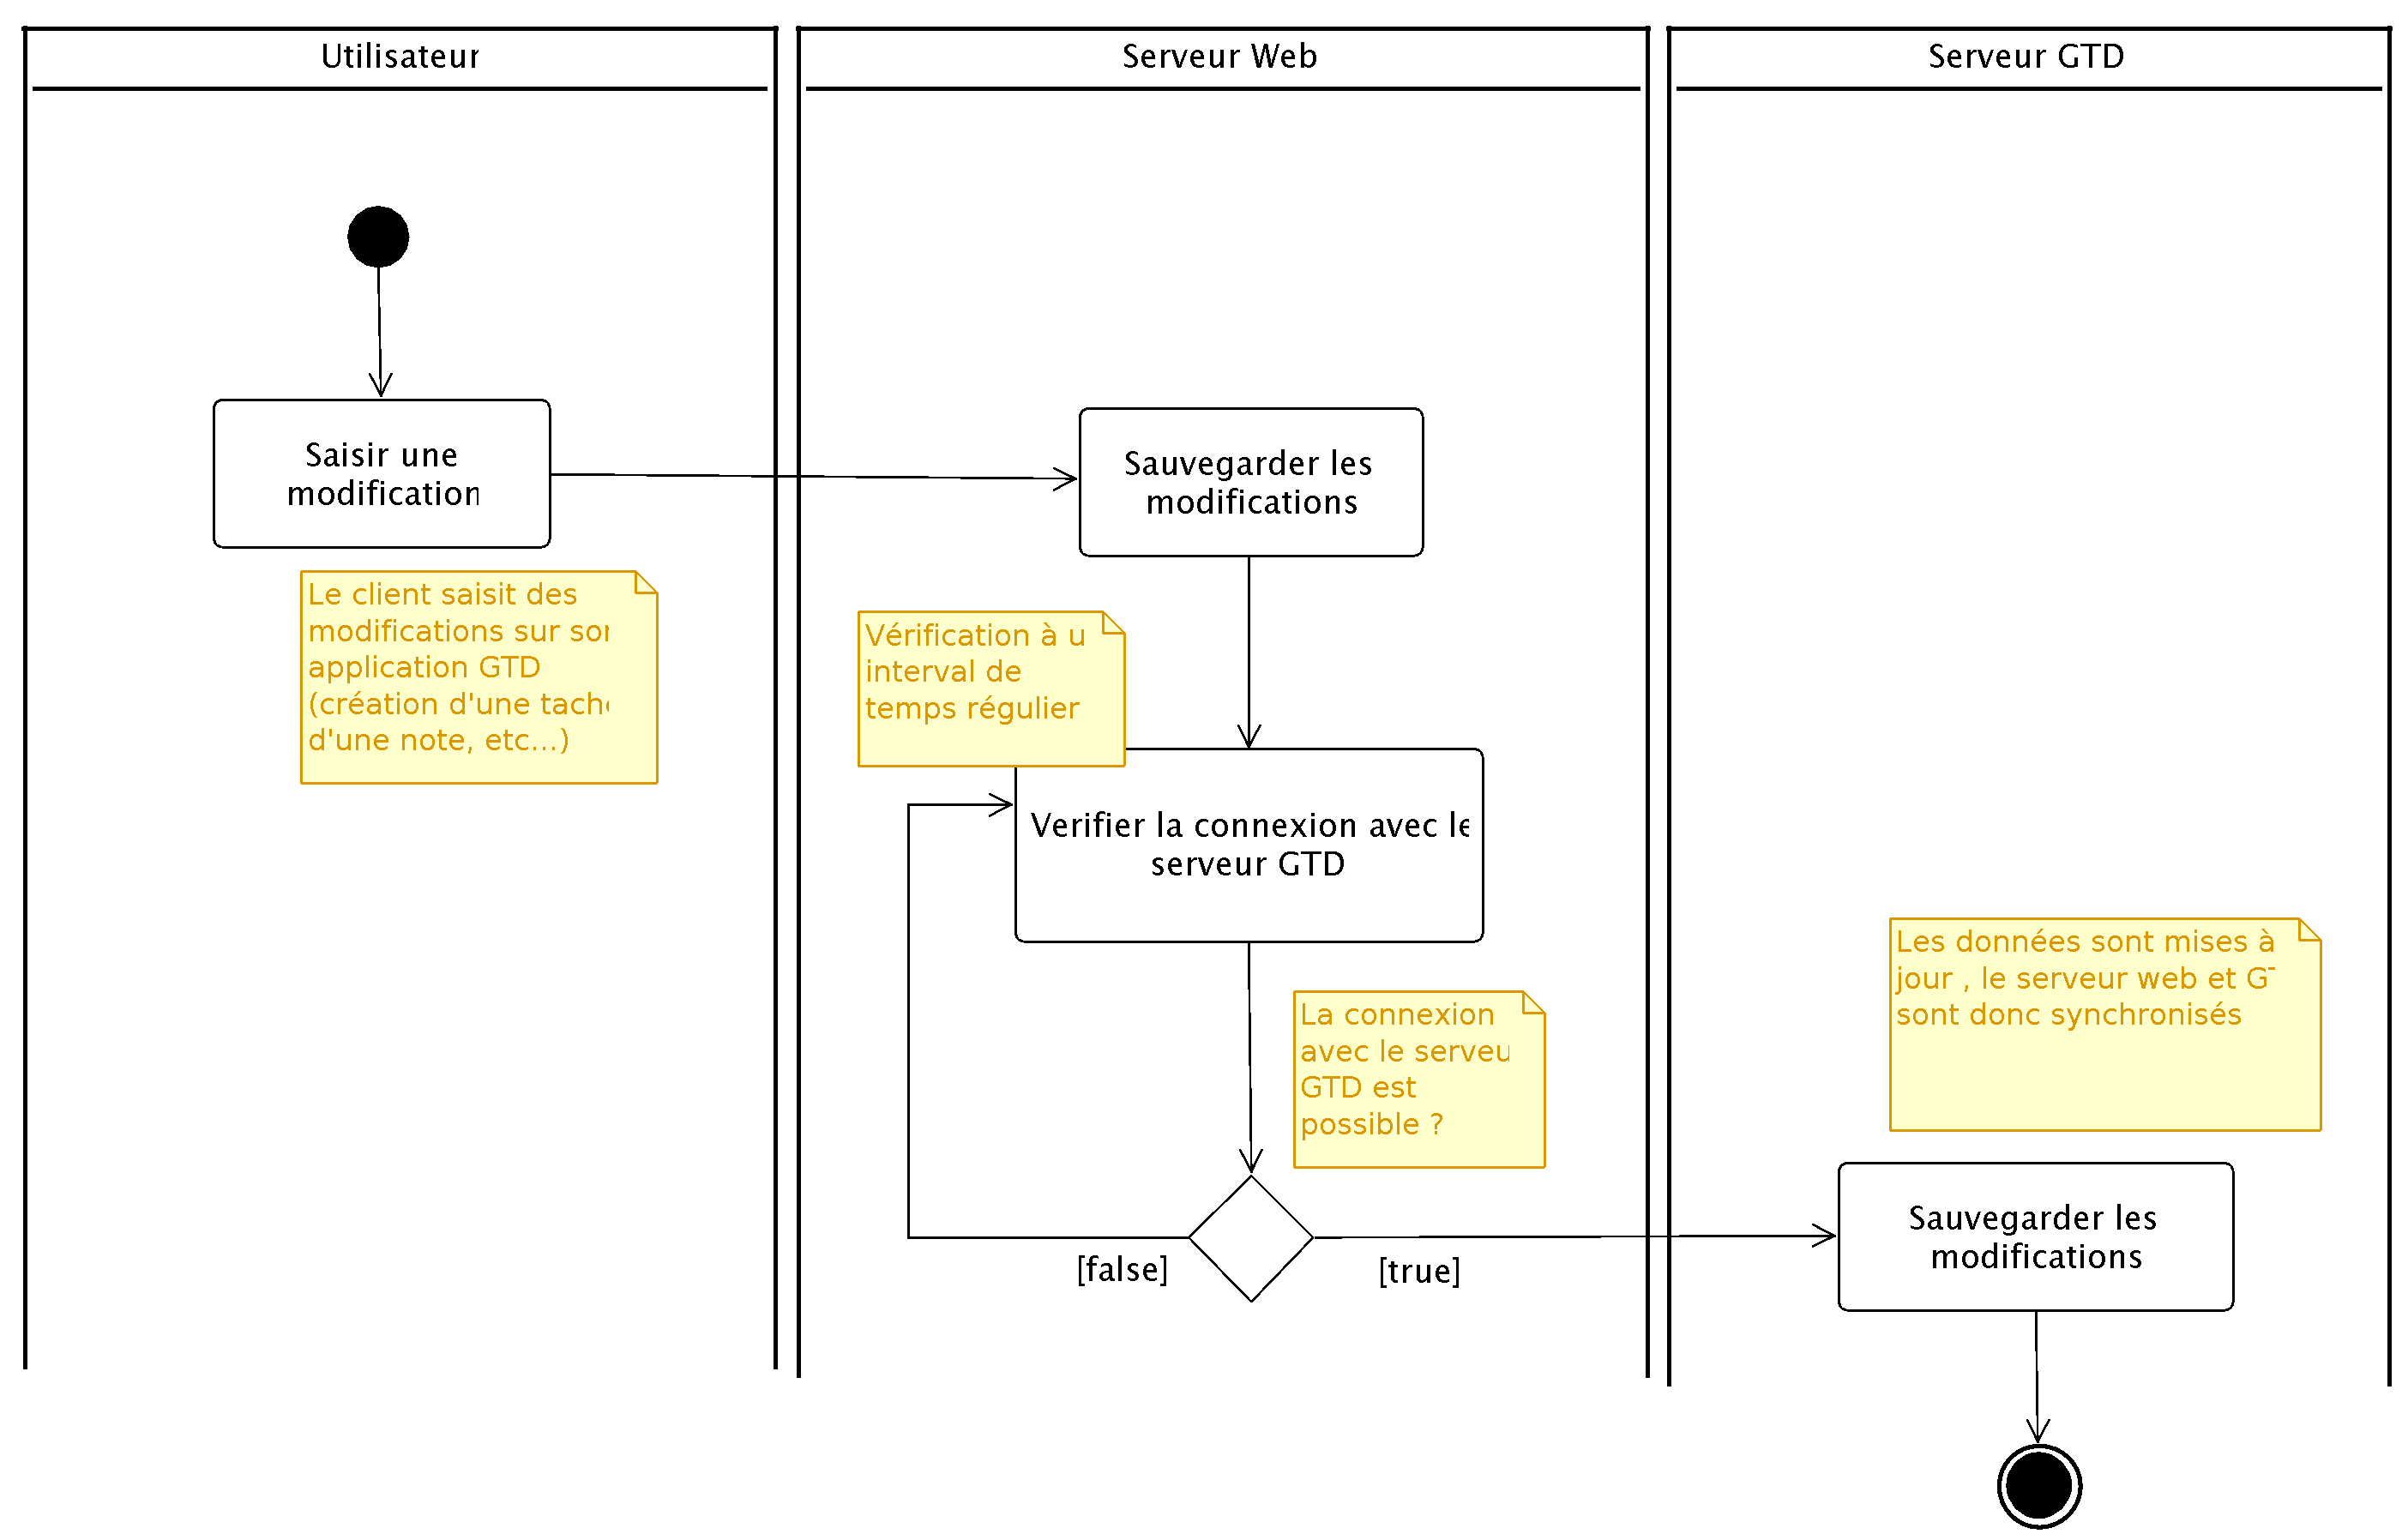
\includegraphics[scale=0.2]{diagrams/activiteSynch.png}
  \caption{UML - Diagramme d'activitées - Synchronisation}
  \label{fig:Architecture Generale}
  \end{center}
  \end{figure}

\subsubsection{Exigences fonctionnelles}
%<Itemize the detailed functional requirements associated with this feature. These are the software capabilities that must be present in order for the user to carry out the services provided by the feature, or to execute the use case. Include how the product should respond to anticipated error conditions or invalid inputs. Requirements should be concise, complete, unambiguous, verifiable, and necessary. Use “TBD” as a placeholder to indicate when necessary information is not yet available.>

%<Each requirement should be uniquely identified with a sequence number or a meaningful tag of some kind.>

%REQ-1:	
%REQ-2:
\begin{itemize}	\renewcommand{\labelitemi}{}
	\item \textbf{FONC61} - Enregistrement des modifications sur le serveur web,
	\item \textbf{FONC62} - Enregistrement des modifications sur les serveurs GTD et ToodleDo
	\item \textbf{FONC63} - Enregistrement des modifications sur les serveurs GTD et ToodleDo après une perte de connexion
\end{itemize}
		


\chapter{Etape 3 : Conception initiale de l’interface}



\section{Modèle de navigation}
L'application doit fournir les fonctionnalités de la méthode GTD qui défini 5 grandes étapes.L'interface graphique a donc été construite autour de celles-ci. En effet, au lancement de l'application, on remarque un axe principal ou les 5 étapes apparaissent clairement. Des flèches rappelle l'ordre chronologique dans lequel elles sont sensées être effectuées. L'utilisateur reste cependant libre de cliquer sur l'étape qu'il souhaite effectuer à tout moment.

%De manière à respecter la méthode GTD, la navigation se fait autour des activités de la méthode. Ainsi la navigation se fait de naturellement de manière séquentielle. Cependant, l'utilisateur reste libre de ses choix et peut facilement changer d'activité. La navigation s'organise autour d'une barre située en haut de l'IHM.%


\section{Look and Field}
L'apparence de l'application est relativement sobre. Ainsi, le nombre de couleurs est limité afin d'offrir un rendu clair et fonctionnel. L'ensemble des éléments graphiques reste simple mais travaillé. Etant donné que nous utilisons GWT, les boutons, les tableaux, et les autres éléments ont tous le même style graphique défini par défaut dans GWT. Le thème général est cependant en adéquation avec ce thème par défaut utilisés par les boutons. Ceux-ci sont correctement placé dans l'interface de façon a ce que l'utilisateur soit efficace dans ses opérations. Les éléments cliquables sont signalés, tout comme chaque élément autorisant une interaction avec l'utilisateur.

L'application réalisée est de type RIA (Rich Internet Application).Elle possède donc les caractéristiques similaires aux logiciels traditionnels installés sur un ordinateur. L'interactivité est est aussi développée que dans une application de bureau et la vitesse d'exécution est particulièrement rapide grâce au framework GWT qui optimise le code javascript de l'application cliente.


\section{Rapidité d'exécution}
Etant donné que l'application est réalisée en GWT, elle offre une réactivité particulièrement intéressante. Le logiciel se comporte comme une application de bureau standard. Lors des actions nécessitant un temps de réalisation plus long, l'utilisateur est cependant informé du temps restant via une barre de progression.


\section{Maquette de l'IHM}

Afin de faciliter le développement de l'IHM, les maquettes suivantes ont étés réalisées. Elles s'organisent autour des principales étapes de la méthode GTD.

\subsection{Connexion à l'application}
Au lancement de l'application l'utilisateur doit pouvoir effectuer toutes les
étapes de la méthode GTD. Cependant, la connexion est indispensable à chacune
des étapes suivantes. En effet, les données sont stockées dans un compte
distant identifié par un login et protégé par un mot de passe. L'interface
suivante permet donc de se connecter, s'inscrire et renvoyer son mot de passe
en cas de perte de celui-ci.

\begin{figure}[H]
  \begin{center}
  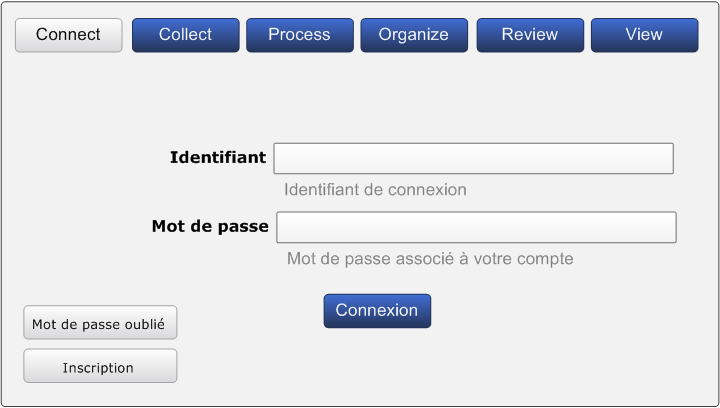
\includegraphics[scale=0.5]{diagrams/connect.png}
  \caption{Mockup - Connection}
  \end{center}
\end{figure}

Une fois que l'utilisateur est connecté, il peut effectuer toutes les étapes 
de la méthode GTD, ou seulement celle qui l'intéresse. L'utilisateur doit
en effet être libre de choisir ce qu'il veux faire au moment où il lance
l'application. Il peut donc le faire par l'axe présent en haut de
l'interface, présentant dans l'ordre chronologique les différentes étapes.

\subsection{Collecte des informations}
Après avoir cliqué sur l'onglet Collect, l'utilisateur dispose d'une interface offrant
les fonctionnalités d'un pense-bête. En effet, Collect est une réflexion de
l'utilisateur, la seule aide que pour fournir l'application est un stockage des
idées n'ayant pas eu le temps d'être traité dans Process. Il peut donc ajouter (bouton +) et supprimer (bouton -) simplement des idées, ici sous forme de post-it.


\begin{figure}[H]
  \begin{center}
  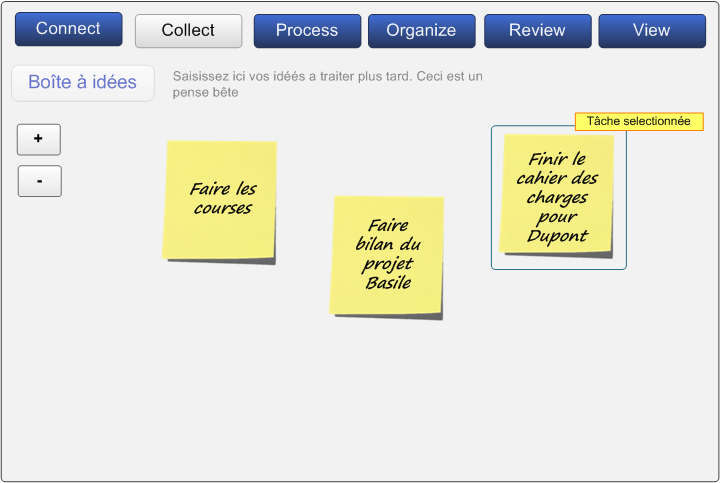
\includegraphics[scale=0.5]{diagrams/collect.png}
  \caption{Mockup - Collect}
  \end{center}
\end{figure}

\subsection{Création des tâches}
Lorsque l'utilisateur clique sur process, il dispose d'une interface affichant
les idées qu'il a actuellement dans son pense-bête et d'une interface de saisie
de tâches. Il peut donc aisément créer ses tâches avec toutes les informations
nécessaires sans oublier celles qui sont dans son pense-bête.


\begin{figure}[H]
  \begin{center}
  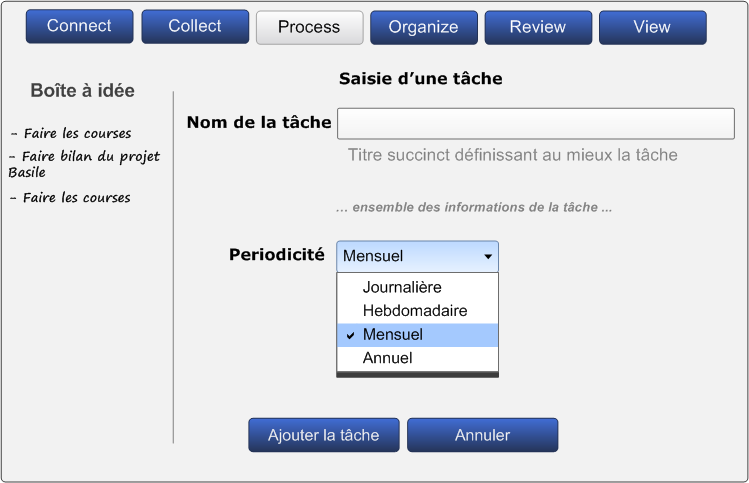
\includegraphics[scale=0.5]{diagrams/process.png}
  \caption{Mockup - Process}
  \end{center}
\end{figure}


\subsection{Organisation des tâches}
Lorsque l'utilisateur clique sur organize, il dispose de deux fonctionnalités :
\begin{itemize}
  \item Organiser les tâches en projet,
  \item Déléguer une tâche.
\end{itemize}
L'organisation inclut la création de projet (bouton +), la définition du
contexte par défaut du projet, ainsi que l'ajout des tâches dans un projet par
glisser-déposer de la liste 'tâches disponibles' vers 'tâches affectées au
projet', en définissant un ordre chronologique.
Pour la délégation il suffit de sélectionner une tâche, puis une personne à qui
déléguer, et enfin de valider.

\begin{figure}[H]
  \begin{center}
  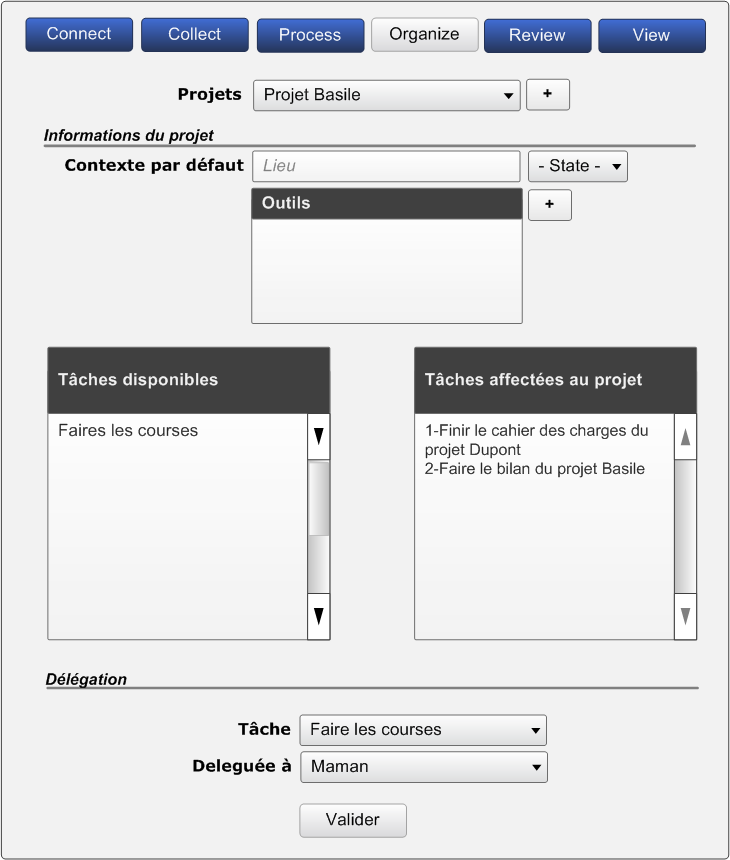
\includegraphics[scale=0.5]{diagrams/organize.png}
  \caption{Mockup - Process}
  \end{center}
\end{figure}

\subsection{Mise à jour des tâches}
L'interface Review permet simplement de mettre à jour les informations de
certaines tâches. Elle correspond donc à l'interface de process.

\begin{figure}[H]
  \begin{center}
  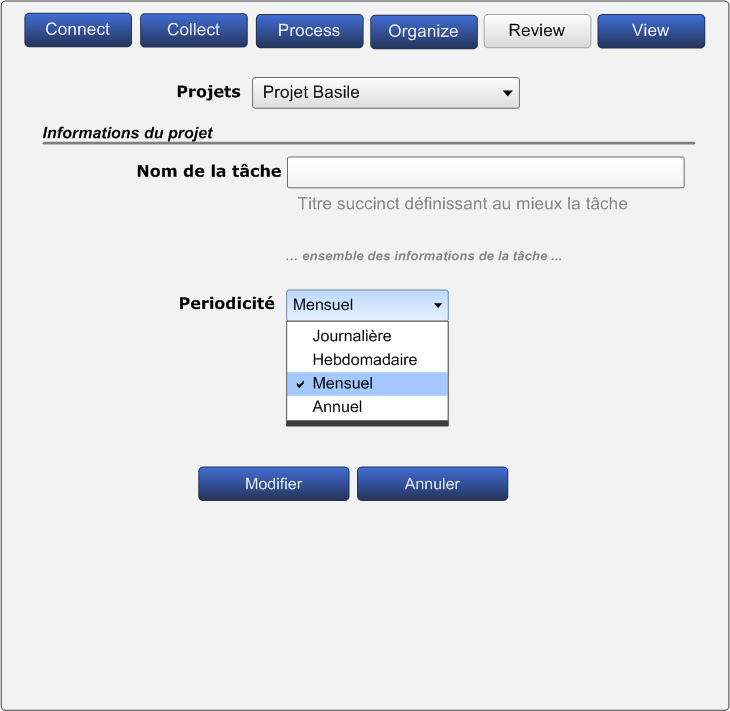
\includegraphics[scale=0.5]{diagrams/review.png}
  \caption{Mockup - Review}
  \end{center}
\end{figure}

\subsection{Visualisation}
La vue est l'opération finale, elle permet d'afficher les tâches en agenda ou
en écheancier afin de conseiller l'utilisateur dans la bonne gestion de son
temps. Le calendrier affiche les jours occupés et la liste des tâches présentes
dans l'ordre de leur priorité depuis la date selectionnée dans le
calendrier.

\begin{figure}[H]
  \begin{center}
  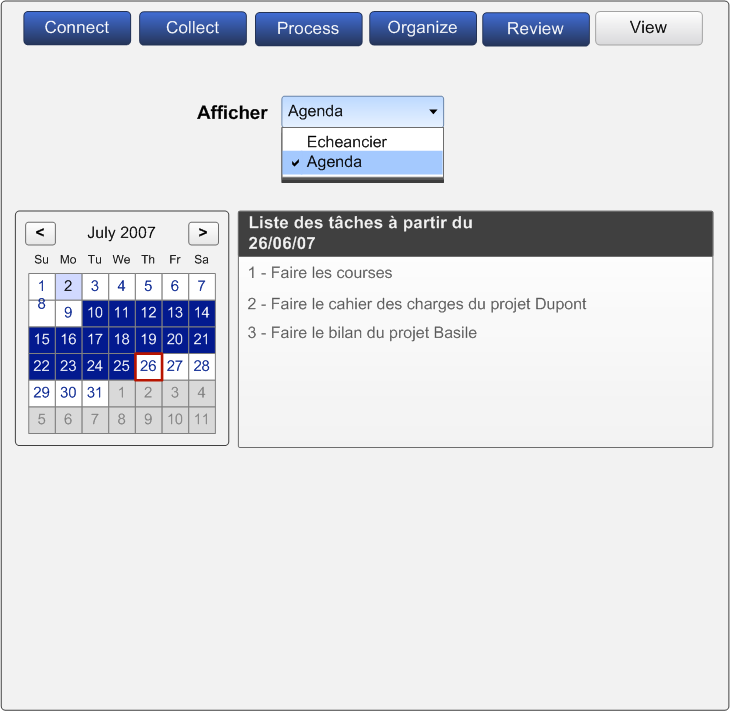
\includegraphics[scale=0.5]{diagrams/view.png}
  \caption{Mockup - View}
  \end{center}
\end{figure}


\chapter{Etape 4 : Développement incrémental}

Comme le montre la figure suivante, nous avons suivi un cycle de développement itératif ou incrémental pour la partie IHM. Chaque cycle est composé des trois étapes suivantes : Conception, Prototypage, Evaluation. Ce mode de développement permet d'avancer rapidement dans le projet en ayant toujours une base fonctionelle et relativement stable. Il est ainsi facile de controler le bon avancement du projet.



\begin{figure}[H]
  \begin{center}
  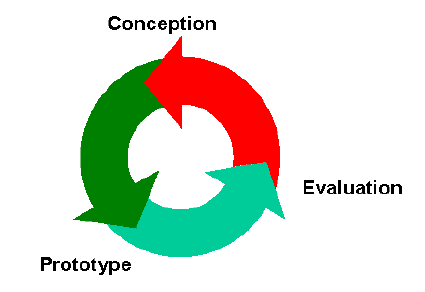
\includegraphics[scale=1]{diagrams/increm.png}
  \caption{Développement incrémental}
  \end{center}
\end{figure}

\chapter{Etape 5 : Implémentation de l’application}

\section{Outils utilisés}
L'IHM est réalisé grâce à la librairie GWT développée par google. Celle ci permet la création simple et rapide d'application AJAX. Elle permet de s'abstraire de la manipulation de javascript et de la gestion des appels asynchrones.



\section{Aide et documentation}
En ce qui concerne la documentation, le programme est livré avec une documentation papier. Celle-ci explique chaque fonction du logiciel en détail, tout en restant claire pour un utilisateur non experimenté\footnote{Par manque de temps celle-ci n'a pu etre finalisée}. De plus, l'IHM dispose de nombreuse bulle d'aide (tooltips) dans le but d'offrir une aide concise et rapide.

\bigskip

Pour ce qui est de l'installation de l'application et du passage de main de celle-ci, une brève formation sera réalisé. Elle sera destiné à l'utilisateur principal du logiciel, ou de son administrateur.


\section{Interface finale}

Voici des impressions écran de l'interface finale, celle-ci reprend l'ensemble des éléments décrit dans ce rapport.
\begin{figure}[H]
  \begin{center}
  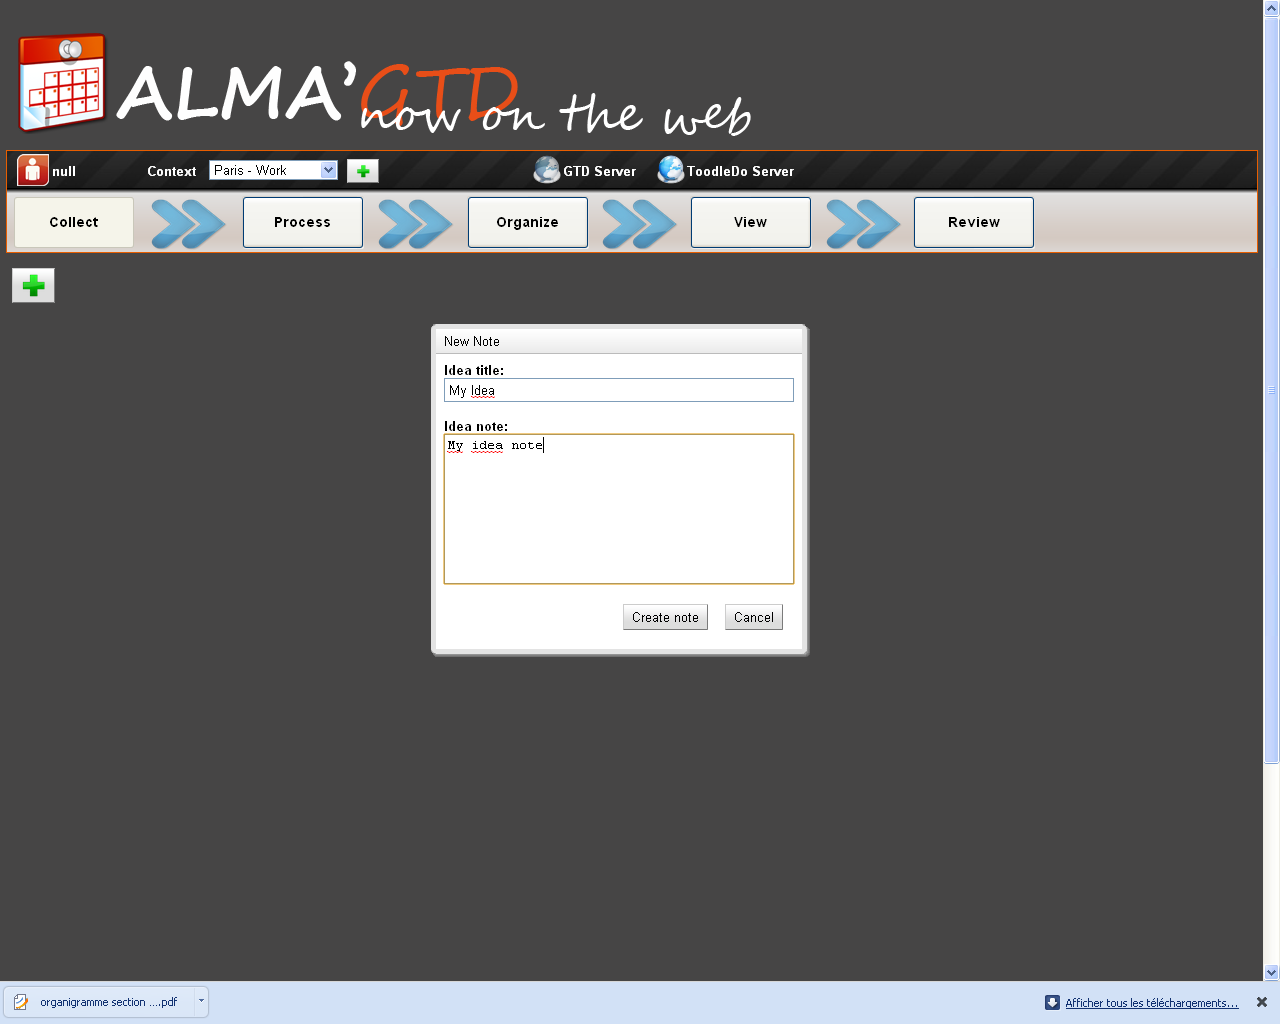
\includegraphics[scale=0.5]{diagrams/D.png}
  \caption{Collecte des informations}
  \end{center}
\end{figure}


\begin{figure}[H]
  \begin{center}
  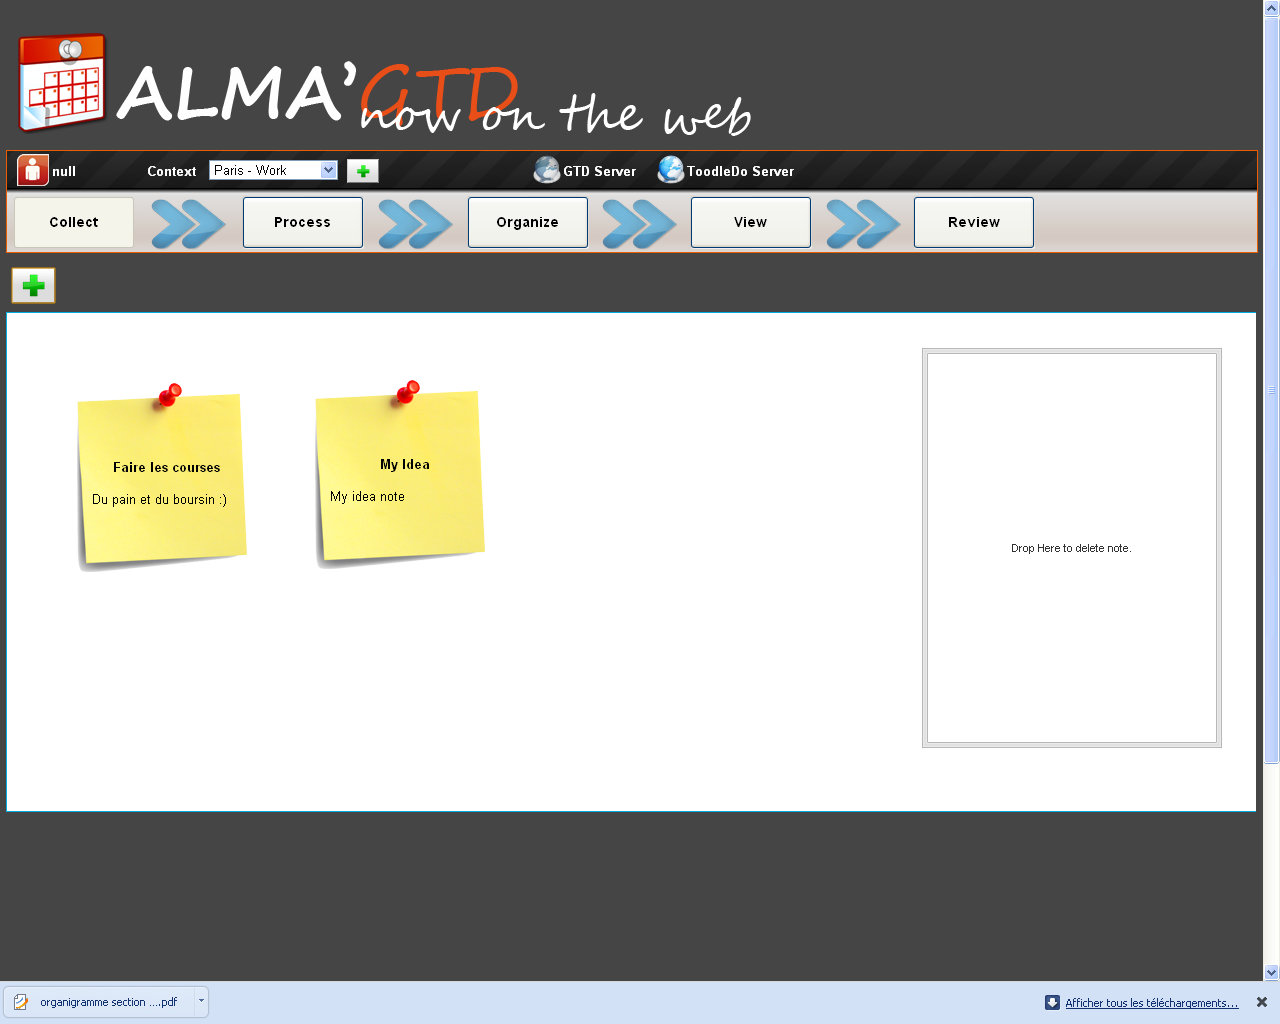
\includegraphics[scale=0.5]{diagrams/C.png}
  \caption{Collecte des informations}
  \end{center}
\end{figure}


\begin{figure}[H]
  \begin{center}
  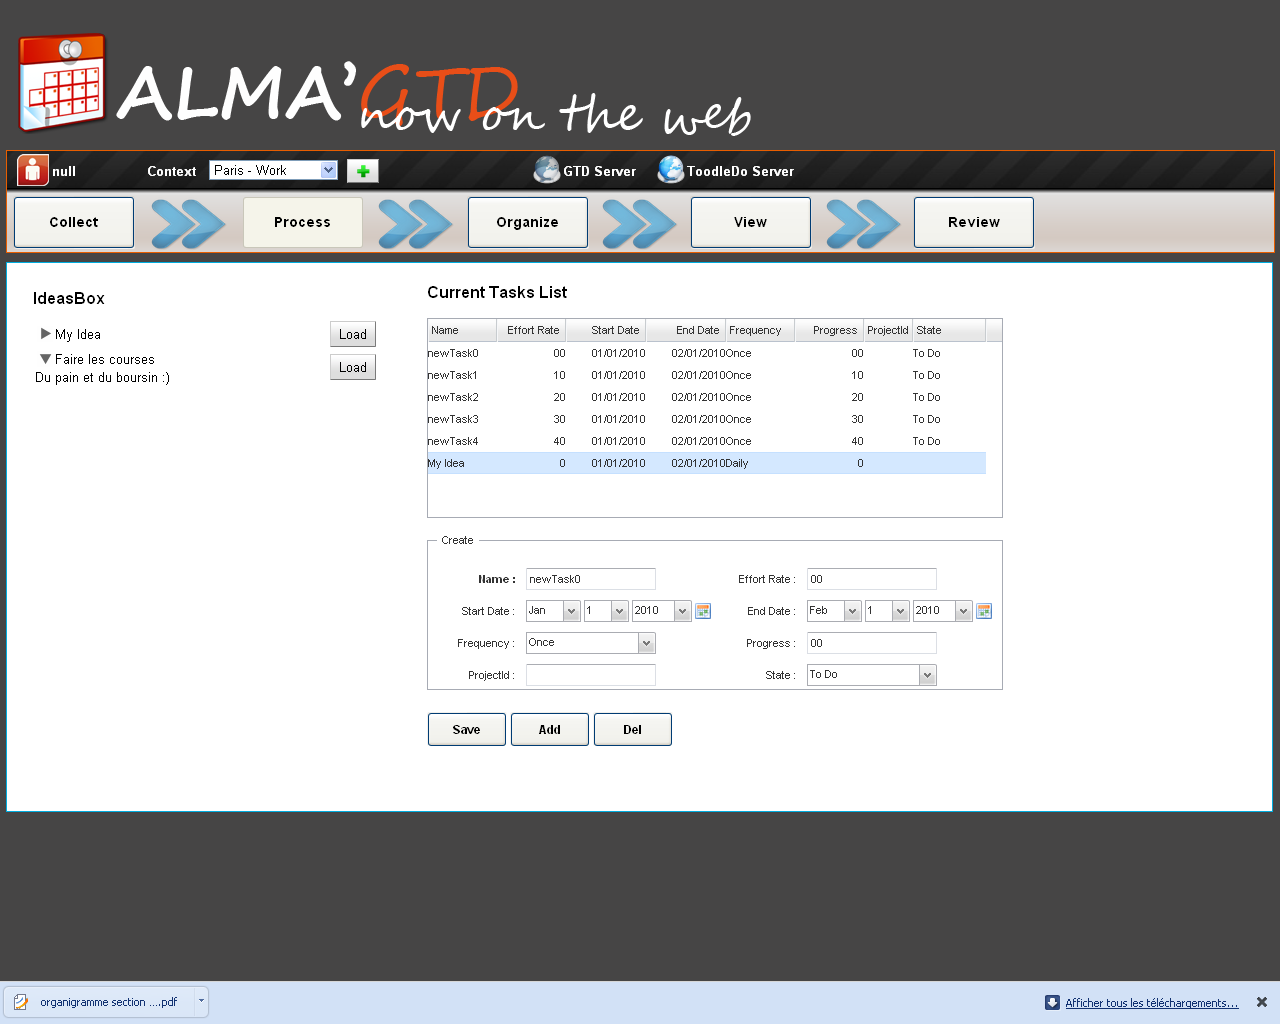
\includegraphics[scale=0.5]{diagrams/B.png}
  \caption{Création des tâches}
  \end{center}
\end{figure}


\begin{figure}[H]
  \begin{center}
  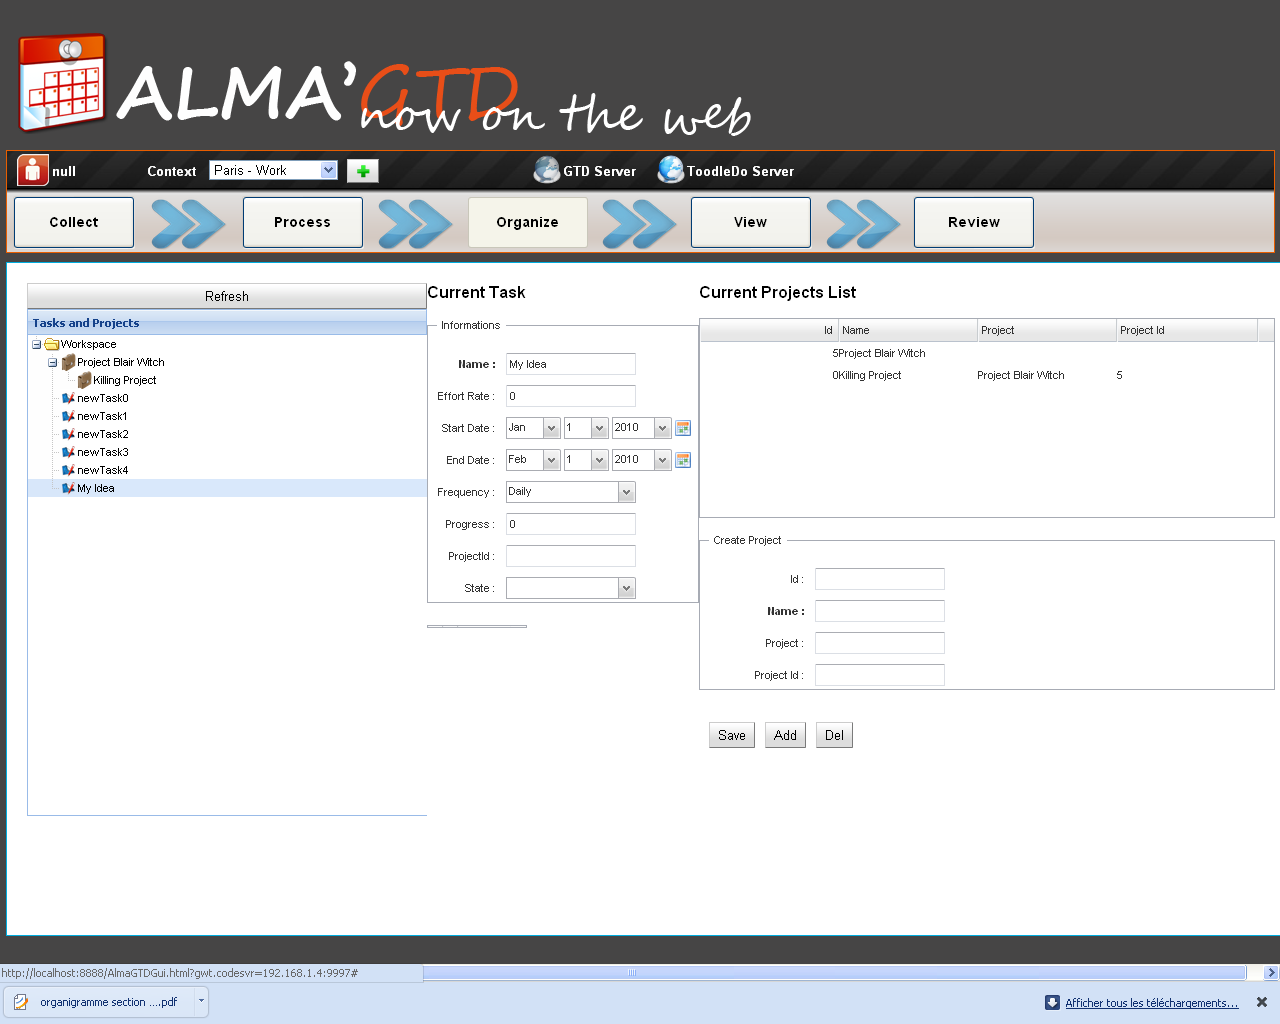
\includegraphics[scale=0.5]{diagrams/A.png}
  \caption{Organisation des tâches}
  \end{center}
\end{figure}

\chapter{Etape 6 : Evaluation externe}
\section{Diffusion d'une version beta}
Dans le but d'aboutir à une version stable, et finalisée. Une première version de test sera mise à disposition des utilisateurs. Celle ci va permettre  de recenser les bugs, et les  problèmes d'utilisation. Cette étape est primordiale car elle permet d'avoir un avis externe à celui de l'équipe de développement. Les bugs seront tous corrigés avant la diffusion d'une autre version de test\footnote{Diffusion d'une RC1 et éventuellement d'une RC2}

\section{Bug repporting}
Le principal moyen de bug repporting se fera via internet et le site du projet\footnote{http://code.google.com/p/almagtd/issues/list}. Toujours via ce site, les utilisateurs ont la possibilité de discuter avec l'équipe de développeurs et peuvent donc faire part de leurs avis.


\chapter{Conclusion}
La réalisation de ce  projet a été particulièrement intéressante pour nous. Bien que nous avons déja eu des cours d'IHM par le passé, nous n'avons jamais utilisé GWT. Cette technologie c'est révélée très puissante pour le développement d'applications Web de par la compatibilité et l'optimisation qu'elle offre pour le client. Il n'est en effet plus nécessaire de manipuler du javascript et de se heurter aux nombreux problèmes de compatibilité avec les navigateurs, bêtes noires du développement Web actuel. De plus, GWT est un framework extrêmement efficace lorsqu'on la pris en main.
\medskip

D'autre part, la réalisation de ce projet nous à permis de mettre en oeuvre tous les principes de développement d'IHM étudiés en cours. Pour cela, nous avons utilisé la méthode de développement LUCID. Le fait d'avoir réalisé une application Web à également été très positif pour l'ensemble de notre groupe, plus souvent habitué à réaliser des applications en SWING. Grâce à la puissance de GWT, il est désormais possible pour une application Web, de rivaliser avec une application classique.

























